\documentclass[10pt]{article}         %% What type of document you're writing.
\usepackage{graphicx}
\usepackage{hyperref}
\usepackage[dvipsnames]{xcolor}

%%%%% Preamble

%% Packages to use

\usepackage{amsmath,amsfonts,amssymb}   %% AMS mathematics macros

%% Title Information.

\title{Twitter Data Model}
\author{Adolfo Centeno}
%% \date{2 July 2004}           %% By default, LaTeX uses the current date

%%%%% The Document

\begin{document}

\maketitle

\begin{abstract}
This document implements the Twitter Data Model.
\end{abstract}

\section{Data Model Description}



\textcolor{red}{Usuarios} de twitter (\textcolor{green}{ idusuario, usuario, email, passwd, telefono, nombre } ) \\
\textcolor{red}{Tweets}  (\textcolor{green}{ idtweet, tweet, urlimagen} ) \\

Los Usuarios \textcolor{yellow}{escribe} Tweets 


\section{E-R Model}

Twitter...

\begin{figure}[h]
     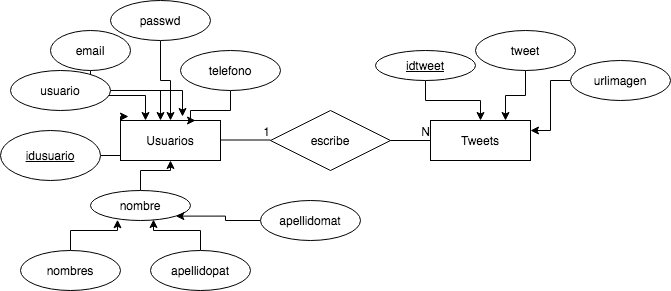
\includegraphics[scale=0.6]{er_twitter}
     \caption{Twitter E-R Model}
\end{figure}
   
\section{Relational Model}
Twitter Relational Model

\begin{figure}[h]
     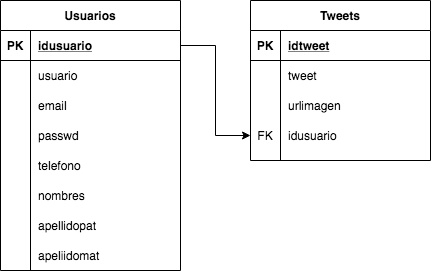
\includegraphics[scale=0.4]{relational_twitter}
     \caption{Twitter Relational Model}
\end{figure}

\end{document}

